
%% bare_conf.tex
%% V1.3
%% 2007/01/11
%% by Michael Shell
%% See:
%% http://www.michaelshell.org/
%% for current contact information.
%%
%% This is a skeleton file demonstrating the use of IEEEtran.cls
%% (requires IEEEtran.cls version 1.7 or later) with an IEEE conference paper.
%%
%% Support sites:
%% http://www.michaelshell.org/tex/ieeetran/
%% http://www.ctan.org/tex-archive/macros/latex/contrib/IEEEtran/
%% and
%% http://www.ieee.org/

%%*************************************************************************
%% Legal Notice:
%% This code is offered as-is without any warranty either expressed or
%% implied; without even the implied warranty of MERCHANTABILITY or
%% FITNESS FOR A PARTICULAR PURPOSE! 
%% User assumes all risk.
%% In no event shall IEEE or any contributor to this code be liable for
%% any damages or losses, including, but not limited to, incidental,
%% consequential, or any other damages, resulting from the use or misuse
%% of any information contained here.
%%
%% All comments are the opinions of their respective authors and are not
%% necessarily endorsed by the IEEE.
%%
%% This work is distributed under the LaTeX Project Public License (LPPL)
%% ( http://www.latex-project.org/ ) version 1.3, and may be freely used,
%% distributed and modified. A copy of the LPPL, version 1.3, is included
%% in the base LaTeX documentation of all distributions of LaTeX released
%% 2003/12/01 or later.
%% Retain all contribution notices and credits.
%% ** Modified files should be clearly indicated as such, including  **
%% ** renaming them and changing author support contact information. **
%%
%% File list of work: IEEEtran.cls, IEEEtran_HOWTO.pdf, bare_adv.tex,
%%                    bare_conf.tex, bare_jrnl.tex, bare_jrnl_compsoc.tex
%%*************************************************************************

% *** Authors should verify (and, if needed, correct) their LaTeX system  ***
% *** with the testflow diagnostic prior to trusting their LaTeX platform ***
% *** with production work. IEEE's font choices can trigger bugs that do  ***
% *** not appear when using other class files.                            ***
% The testflow support page is at:
% http://www.michaelshell.org/tex/testflow/



% Note that the a4paper option is mainly intended so that authors in
% countries using A4 can easily print to A4 and see how their papers will
% look in print - the typesetting of the document will not typically be
% affected with changes in paper size (but the bottom and side margins will).
% Use the testflow package mentioned above to verify correct handling of
% both paper sizes by the user's LaTeX system.
%
% Also note that the "draftcls" or "draftclsnofoot", not "draft", option
% should be used if it is desired that the figures are to be displayed in
% draft mode.
%
\documentclass[conference]{IEEEtran}
% Add the compsoc option for Computer Society conferences.
%
% If IEEEtran.cls has not been installed into the LaTeX system files,
% manually specify the path to it like:
% \documentclass[conference]{../sty/IEEEtran}





% Some very useful LaTeX packages include:
% (uncomment the ones you want to load)


% *** MISC UTILITY PACKAGES ***
%
%\usepackage{ifpdf}
% Heiko Oberdiek's ifpdf.sty is very useful if you need conditional
% compilation based on whether the output is pdf or dvi.
% usage:
% \ifpdf
%   % pdf code
% \else
%   % dvi code
% \fi
% The latest version of ifpdf.sty can be obtained from:
% http://www.ctan.org/tex-archive/macros/latex/contrib/oberdiek/
% Also, note that IEEEtran.cls V1.7 and later provides a builtin
% \ifCLASSINFOpdf conditional that works the same way.
% When switching from latex to pdflatex and vice-versa, the compiler may
% have to be run twice to clear warning/error messages.






% *** CITATION PACKAGES ***
%
%\usepackage{cite}
% cite.sty was written by Donald Arseneau
% V1.6 and later of IEEEtran pre-defines the format of the cite.sty package
% \cite{} output to follow that of IEEE. Loading the cite package will
% result in citation numbers being automatically sorted and properly
% "compressed/ranged". e.g., [1], [9], [2], [7], [5], [6] without using
% cite.sty will become [1], [2], [5]--[7], [9] using cite.sty. cite.sty's
% \cite will automatically add leading space, if needed. Use cite.sty's
% noadjust option (cite.sty V3.8 and later) if you want to turn this off.
% cite.sty is already installed on most LaTeX systems. Be sure and use
% version 4.0 (2003-05-27) and later if using hyperref.sty. cite.sty does
% not currently provide for hyperlinked citations.
% The latest version can be obtained at:
% http://www.ctan.org/tex-archive/macros/latex/contrib/cite/
% The documentation is contained in the cite.sty file itself.






% *** GRAPHICS RELATED PACKAGES ***
%
\ifCLASSINFOpdf
  \usepackage[pdftex]{graphicx}
  % declare the path(s) where your graphic files are
  \graphicspath{{../pdf/}{../jpeg/}{figures}}
  % and their extensions so you won't have to specify these with
  % every instance of \includegraphics
  \DeclareGraphicsExtensions{.pdf,.jpeg,.png}
\else
  % or other class option (dvipsone, dvipdf, if not using dvips). graphicx
  % will default to the driver specified in the system graphics.cfg if no
  % driver is specified.
  % \usepackage[dvips]{graphicx}
  % declare the path(s) where your graphic files are
  % \graphicspath{{../eps/}}
  % and their extensions so you won't have to specify these with
  % every instance of \includegraphics
  % \DeclareGraphicsExtensions{.eps}
\fi
% graphicx was written by David Carlisle and Sebastian Rahtz. It is
% required if you want graphics, photos, etc. graphicx.sty is already
% installed on most LaTeX systems. The latest version and documentation can
% be obtained at: 
% http://www.ctan.org/tex-archive/macros/latex/required/graphics/
% Another good source of documentation is "Using Imported Graphics in
% LaTeX2e" by Keith Reckdahl which can be found as epslatex.ps or
% epslatex.pdf at: http://www.ctan.org/tex-archive/info/
%
% latex, and pdflatex in dvi mode, support graphics in encapsulated
% postscript (.eps) format. pdflatex in pdf mode supports graphics
% in .pdf, .jpeg, .png and .mps (metapost) formats. Users should ensure
% that all non-photo figures use a vector format (.eps, .pdf, .mps) and
% not a bitmapped formats (.jpeg, .png). IEEE frowns on bitmapped formats
% which can result in "jaggedy"/blurry rendering of lines and letters as
% well as large increases in file sizes.
%
% You can find documentation about the pdfTeX application at:
% http://www.tug.org/applications/pdftex





% *** MATH PACKAGES ***
%
%\usepackage[cmex10]{amsmath}
% A popular package from the American Mathematical Society that provides
% many useful and powerful commands for dealing with mathematics. If using
% it, be sure to load this package with the cmex10 option to ensure that
% only type 1 fonts will utilized at all point sizes. Without this option,
% it is possible that some math symbols, particularly those within
% footnotes, will be rendered in bitmap form which will result in a
% document that can not be IEEE Xplore compliant!
%
% Also, note that the amsmath package sets \interdisplaylinepenalty to 10000
% thus preventing page breaks from occurring within multiline equations. Use:
%\interdisplaylinepenalty=2500
% after loading amsmath to restore such page breaks as IEEEtran.cls normally
% does. amsmath.sty is already installed on most LaTeX systems. The latest
% version and documentation can be obtained at:
% http://www.ctan.org/tex-archive/macros/latex/required/amslatex/math/





% *** SPECIALIZED LIST PACKAGES ***
%
%\usepackage{algorithmic}
% algorithmic.sty was written by Peter Williams and Rogerio Brito.
% This package provides an algorithmic environment fo describing algorithms.
% You can use the algorithmic environment in-text or within a figure
% environment to provide for a floating algorithm. Do NOT use the algorithm
% floating environment provided by algorithm.sty (by the same authors) or
% algorithm2e.sty (by Christophe Fiorio) as IEEE does not use dedicated
% algorithm float types and packages that provide these will not provide
% correct IEEE style captions. The latest version and documentation of
% algorithmic.sty can be obtained at:
% http://www.ctan.org/tex-archive/macros/latex/contrib/algorithms/
% There is also a support site at:
% http://algorithms.berlios.de/index.html
% Also of interest may be the (relatively newer and more customizable)
% algorithmicx.sty package by Szasz Janos:
% http://www.ctan.org/tex-archive/macros/latex/contrib/algorithmicx/




% *** ALIGNMENT PACKAGES ***
%
%\usepackage{array}
% Frank Mittelbach's and David Carlisle's array.sty patches and improves
% the standard LaTeX2e array and tabular environments to provide better
% appearance and additional user controls. As the default LaTeX2e table
% generation code is lacking to the point of almost being broken with
% respect to the quality of the end results, all users are strongly
% advised to use an enhanced (at the very least that provided by array.sty)
% set of table tools. array.sty is already installed on most systems. The
% latest version and documentation can be obtained at:
% http://www.ctan.org/tex-archive/macros/latex/required/tools/


%\usepackage{mdwmath}
%\usepackage{mdwtab}
% Also highly recommended is Mark Wooding's extremely powerful MDW tools,
% especially mdwmath.sty and mdwtab.sty which are used to format equations
% and tables, respectively. The MDWtools set is already installed on most
% LaTeX systems. The lastest version and documentation is available at:
% http://www.ctan.org/tex-archive/macros/latex/contrib/mdwtools/


% IEEEtran contains the IEEEeqnarray family of commands that can be used to
% generate multiline equations as well as matrices, tables, etc., of high
% quality.


%\usepackage{eqparbox}
% Also of notable interest is Scott Pakin's eqparbox package for creating
% (automatically sized) equal width boxes - aka "natural width parboxes".
% Available at:
% http://www.ctan.org/tex-archive/macros/latex/contrib/eqparbox/





% *** SUBFIGURE PACKAGES ***
%\usepackage[tight,footnotesize]{subfigure}
% subfigure.sty was written by Steven Douglas Cochran. This package makes it
% easy to put subfigures in your figures. e.g., "Figure 1a and 1b". For IEEE
% work, it is a good idea to load it with the tight package option to reduce
% the amount of white space around the subfigures. subfigure.sty is already
% installed on most LaTeX systems. The latest version and documentation can
% be obtained at:
% http://www.ctan.org/tex-archive/obsolete/macros/latex/contrib/subfigure/
% subfigure.sty has been superceeded by subfig.sty.



%\usepackage[caption=false]{caption}
%\usepackage[font=footnotesize]{subfig}
% subfig.sty, also written by Steven Douglas Cochran, is the modern
% replacement for subfigure.sty. However, subfig.sty requires and
% automatically loads Axel Sommerfeldt's caption.sty which will override
% IEEEtran.cls handling of captions and this will result in nonIEEE style
% figure/table captions. To prevent this problem, be sure and preload
% caption.sty with its "caption=false" package option. This is will preserve
% IEEEtran.cls handing of captions. Version 1.3 (2005/06/28) and later 
% (recommended due to many improvements over 1.2) of subfig.sty supports
% the caption=false option directly:
%\usepackage[caption=false,font=footnotesize]{subfig}
%
% The latest version and documentation can be obtained at:
% http://www.ctan.org/tex-archive/macros/latex/contrib/subfig/
% The latest version and documentation of caption.sty can be obtained at:
% http://www.ctan.org/tex-archive/macros/latex/contrib/caption/




% *** FLOAT PACKAGES ***
%
%\usepackage{fixltx2e}
% fixltx2e, the successor to the earlier fix2col.sty, was written by
% Frank Mittelbach and David Carlisle. This package corrects a few problems
% in the LaTeX2e kernel, the most notable of which is that in current
% LaTeX2e releases, the ordering of single and double column floats is not
% guaranteed to be preserved. Thus, an unpatched LaTeX2e can allow a
% single column figure to be placed prior to an earlier double column
% figure. The latest version and documentation can be found at:
% http://www.ctan.org/tex-archive/macros/latex/base/



%\usepackage{stfloats}
% stfloats.sty was written by Sigitas Tolusis. This package gives LaTeX2e
% the ability to do double column floats at the bottom of the page as well
% as the top. (e.g., "\begin{figure*}[!b]" is not normally possible in
% LaTeX2e). It also provides a command:
%\fnbelowfloat
% to enable the placement of footnotes below bottom floats (the standard
% LaTeX2e kernel puts them above bottom floats). This is an invasive package
% which rewrites many portions of the LaTeX2e float routines. It may not work
% with other packages that modify the LaTeX2e float routines. The latest
% version and documentation can be obtained at:
% http://www.ctan.org/tex-archive/macros/latex/contrib/sttools/
% Documentation is contained in the stfloats.sty comments as well as in the
% presfull.pdf file. Do not use the stfloats baselinefloat ability as IEEE
% does not allow \baselineskip to stretch. Authors submitting work to the
% IEEE should note that IEEE rarely uses double column equations and
% that authors should try to avoid such use. Do not be tempted to use the
% cuted.sty or midfloat.sty packages (also by Sigitas Tolusis) as IEEE does
% not format its papers in such ways.





% *** PDF, URL AND HYPERLINK PACKAGES ***
%
%\usepackage{url}
% url.sty was written by Donald Arseneau. It provides better support for
% handling and breaking URLs. url.sty is already installed on most LaTeX
% systems. The latest version can be obtained at:
% http://www.ctan.org/tex-archive/macros/latex/contrib/misc/
% Read the url.sty source comments for usage information. Basically,
% \url{my_url_here}.





% *** Do not adjust lengths that control margins, column widths, etc. ***
% *** Do not use packages that alter fonts (such as pslatex).         ***
% There should be no need to do such things with IEEEtran.cls V1.6 and later.
% (Unless specifically asked to do so by the journal or conference you plan
% to submit to, of course. )


% correct bad hyphenation here
\hyphenation{vis-ual lang-u-ages}


\begin{document}
%
% paper title
% can use linebreaks \\ within to get better formatting as desired
\title{Measuring the Programmatic Complexity of Projects of Varying Functionality in App Inventor}


% author names and affiliations
% use a multiple column layout for up to three different
% affiliations
\author{\IEEEauthorblockN{Benjamin Xie, Isra Shabir, and Hal Abelson}
\IEEEauthorblockA{Department of Electrical Engineering and Computer Science\\
Massachusetts Institute of Technology\\
Cambridge, Massachusetts, USA\\
Email: \{bxie, ishabir, hal\}@mit.edu}}
%\and
%\IEEEauthorblockN{Isra Shabir}
%\IEEEauthorblockA{Department of Electrical Engineering\\and Computer Science\\
%Massachusetts Institute of Technology\\
%Cambridge, Massachusetts 02139\\
%Email: ishabir@mit.edu}
%\and
%\IEEEauthorblockN{James Kirk\\ and Montgomery Scott}
%\IEEEauthorblockA{Starfleet Academy\\
%San Francisco, California 96678-2391\\
%Telephone: (800) 555--1212\\
%Fax: (888) 555--1212}}

% conference papers do not typically use \thanks and this command
% is locked out in conference mode. If really needed, such as for
% the acknowledgment of grants, issue a \IEEEoverridecommandlockouts
% after \documentclass

% for over three affiliations, or if they all won't fit within the width
% of the page, use this alternative format:
% 
%\author{\IEEEauthorblockN{Michael Shell\IEEEauthorrefmark{1},
%Homer Simpson\IEEEauthorrefmark{2},
%James Kirk\IEEEauthorrefmark{3}, 
%Montgomery Scott\IEEEauthorrefmark{3} and
%Eldon Tyrell\IEEEauthorrefmark{4}}
%\IEEEauthorblockA{\IEEEauthorrefmark{1}School of Electrical and Computer Engineering\\
%Georgia Institute of Technology,
%Atlanta, Georgia 30332--0250\\ Email: see http://www.michaelshell.org/contact.html}
%\IEEEauthorblockA{\IEEEauthorrefmark{2}Twentieth Century Fox, Springfield, USA\\
%Email: homer@thesimpsons.com}
%\IEEEauthorblockA{\IEEEauthorrefmark{3}Starfleet Academy, San Francisco, California 96678-2391\\
%Telephone: (800) 555--1212, Fax: (888) 555--1212}
%\IEEEauthorblockA{\IEEEauthorrefmark{4}Tyrell Inc., 123 Replicant Street, Los Angeles, California 90210--4321}}




% use for special paper notices
%\IEEEspecialpapernotice{(Invited Paper)}




% make the title area
\maketitle


\begin{abstract}
%\boldmath
MIT App Inventor is a visual blocks language that enables users with little to no previous programming experience to create applications for Android devices. We analyze a random sampling of projects to better understand what apps the App Inventor environment lends itself towards creating. In particular, we group projects of similar functionality and measure the programmatic complexity of these projects.\end{abstract}
% IEEEtran.cls defaults to using nonbold math in the Abstract.
% This preserves the distinction between vectors and scalars. However,
% if the conference you are submitting to favors bold math in the abstract,
% then you can use LaTeX's standard command \boldmath at the very start
% of the abstract to achieve this. Many IEEE journals/conferences frown on
% math in the abstract anyway.

% no keywords




% For peer review papers, you can put extra information on the cover
% page as needed:
% \ifCLASSOPTIONpeerreview
% \begin{center} \bfseries EDICS Category: 3-BBND \end{center}
% \fi
%
% For peerreview papers, this IEEEtran command inserts a page break and
% creates the second title. It will be ignored for other modes.
\IEEEpeerreviewmaketitle



\section{Introduction}

% no \IEEEPARstart


% You must have at least 2 lines in the paragraph with the drop letter
% (should never be an issue)


%\hfill mds
 
%\hfill April 3, 2015

%\subsection{MIT App Inventor}
MIT App Inventor is an environment that leverages a blocks-based visual programming language to create mobile apps for Android devices. A project consists of a set of components and a set of blocks which give the components functionality. Components include visual items (e.g. buttons, text boxes, images, drawing canvas) as well as non-visible items (e.g. camera, accelerometer, speech recognizer, GPS location sensor). The app's functionality is programmed in Blockly, a visual blocks-based programming language. Figure 1 shows blocks for an app to prevent texting while driving. When a text is received, a predefined message is sent back to the person who sent the original text. 

\begin{figure}[h!]
	\centering
	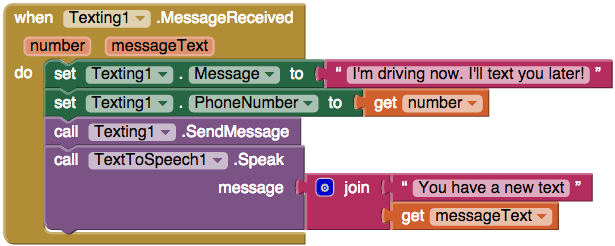
\includegraphics[width=0.95\linewidth]{fig1.png}
	\caption{Blocks for an app that automatically responds to texts received with a predefined message.}
	\label{FIgure 1: Label}
\end{figure}

There have been two major versions of App Inventor. App Inventor Classic (also known as App Inventor 1) was released in 2009 and ran the blocks editor from a separate Java application. In late 2013, App Inventor 2 was released; the blocks editor now runs in a web browser in  as a Javascript program. Although both versions of App Inventor are currently still in use, as of February 2015, 90\% of App Inventor users use App Inventor 2. For this reason, the research here focuses on App Inventor 2 data.

To date, over 3.1 million users from 195 countries have created over 8.2 million projects. There are over 100,000 weekly users. We seek to better understand what users create with App Inventor and determine what kinds of apps the App Inventor environment lends itself towards creating. To do this, we analyze the types of apps created and the programmatic complexity of the projects from a random sample of projects. We group apps of similar functionality based on the components used in the app. To measure programmatic complexity, we assign each block a score where a higher score suggests more advanced programming. We then look at the unique blocks in a project and average the complexity score of each block to determine the complexity of the app.

\subsection{Defining Programmatic Complexity}
TODO

\subsection{Previous Work}
Previous analysis of App Inventor Classic was done mostly at a user level. Notable findings:
\begin{itemize}
	\item 30\% of projects have no blocks and therefore are not functional.
	\item Nearly 50\% of users do not have a single block or component in their projects
	\item 53\% of users only have 1 project.
\end{itemize}
From this, we gather that a significant amount of App Inventor Classic projects were never completed. It was theorized that a major contributing factor is the usability of the service. Whereas App inventor 2 is a single-page web service, App Inventor Classic required the deployment of an external Java service to program the app. Furthermore, the block language was overhauled and improved between versions of App Inventor.

App Inventor is taught at both a grade school and college level, to a diverse audience. Reports on courses taught depict App Inventor being used to create very diverse apps. These apps range from apps that discourage texting while driving to apps that track school buses to apps that organize community service cleanups. The pattern we see is that App Inventor enables "situated computing." This quarter-century old concept suggests that the convergence of computing, connectivity, and content enables users to use computing to bridge the gap between intentions and actions. App Inventor enables users to leverage their mobile devices to solve the problems everyday problems they encounter.

\section{Technical Approach}

We extract features from a random sampling of App Inventor 2 projects. We group projects based on the functionality of their components and also assign a complexity score based on the number of unique blocks in the project and a weighting system that considers the complexity of each block. From there, we look at each group and the distribution of the projects by complexity.

\subsection{Data Source}
Our source data is 5,228 random App Inventor 2 projects. We randomly selected projects according to their project ID, a a sequentially increasing number (so a project with a lesser project ID corresponds to a project made earlier). The 5,228 projects selected come from 5,174 users, suggesting that randomization was accomplished. Given the size of the dataset and the randomness of the selection, we assume that the sample is representative of all App Inventor 2 projects.

Of the 5,228 projects sampled...
\begin{itemize}
	\item 21\% (1,107 projects) are "certainly nonfunctional." That is, these projects either have no components or less than two blocks (the minimum required to have any functionality).
	\item At least 18\% (937 projects) are recreations of tutorials. App Inventor has copious online teaching resources. Most of which consist of a step-by-step guide to creating an app. We find projects that are recreations of fourteen popular tutorials by matching by project name.
	\item 16\% (845 projects) define procedures, suggesting code reuse.
	\item 29\% (1,514 projects) initialize a global variable.
\end{itemize}

\subsection{Feature Extraction}
We focus primarily on quantitative features to enable us to run clustering algorithms. In particular, we look at the number each kind of component in a project, as well as the number of each type of block. The type of a component or block is provided in the source code of the project. 

Features Extracted from Projects:
\begin{itemize}
	\item Project Name
	\item User Name (anonymized)
	\item Number of Screens in Project
	\item Number of Components by Type
	\item Number of Blocks by Type
\end{itemize}


While most block types correspond to exactly one block, there are exceptions. Of particular note are the component blocks. Every component (e.g. button, text box, canvas) that is added to the project has associated blocks to give the component functionality. Although these blocks vary by component, they all correspond to one of three types: Component events, methods, and setter/getters. Component events are outer or top level blocks that run the code within it when the event (e.g. when button clicked) occurs. Component methods are methods relating to the component that can be called (e.g. drawing a point on a canvas). Setter/getter methods are used to either change the component properties (e.g. set the paint color of a canvas) or retrieve the component properties (e.g. text within a text box). Figure 2 provides examples of each of three component block types.

\begin{figure}[h!]
	\centering
	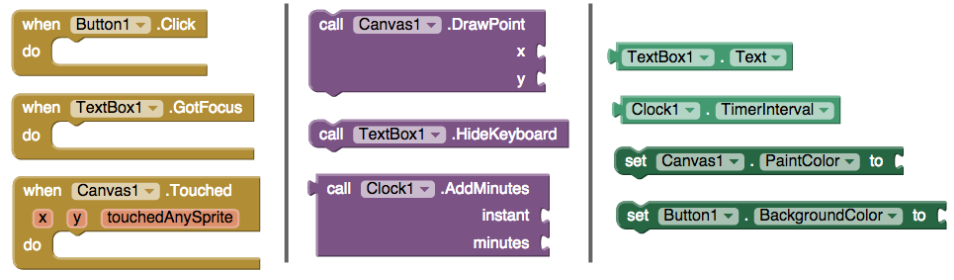
\includegraphics[width=0.95\linewidth]{component_blocks.png}
	\caption{Examples of component blocks of various types. Left Column: "Component Event" blocks. Center Column: "Component Method" blocks. Right Column: "Component Set/Get" blocks.}
	\label{FIgure 2: Component Blocks}
\end{figure}

\subsection{Grouping Projects}
We group projects according to the components they contain. We group projects primarily on the grouping provided in the palette of the designer page in App Inventor 2 (Figure 3). The "User Interface" group contains basic components that almost all apps will use (buttons, text boxes, etc.). The "Layout" group, as it contains components that alter the aesthetics of the app but nothing further. Because layout components do not alter the functionality of projects, they are ignored. The "Media" group contains components that play or record text, sound, pictures, and video. The "Drawing and Animation" group contains components for drawing and basic animations. The "Sensors" group includes components that access the phone's sensors. They include the clock, GPS, and accelerometer. The "Social" group has components to access the phone's contacts, email, calling capability, texting, and Twitter. The "Storage" group is used to persist information. "Connectivity" includes bluetooth and web components to connect to other devices. "Lego Mindstorms" includes components to interface with the programmable Lego robotics kit.

\begin{figure}[h!]
	\centering
	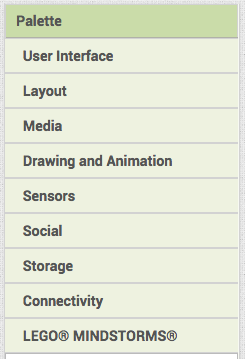
\includegraphics[width=0.4\linewidth]{palette.png}
	\caption{The palette in App Inventor 2 groups components into categories. These categories are used to group projects by functionality}
	\label{FIgure 2: Component Blocks}
\end{figure}

There are eight groups. Basic apps only User Interface components (and possible Layout components, but they are ignored). Media, Drawing, Sensor, Social, Storage, Connectivity, and Lego apps contain at least one component in the respective group in the palette. This categorization allows for overlap, as project that contain components from multiple palette groups may be placed into multiple groups. In example, a project that uses both bluetooth (connectivity) and a twitter (social) component would be labelled both connectivity and social.

\subsection{Measuring Programmatic Complexity}
We look at the number of unique blocks in a project as the primary measure of the programmatic complexity. We choose the number of unique blocks rather than just the number of blocks in a project to account for projects that do not use reuse code when it would be appropriate to do so. 

In example, consider the case where two functionally similar projects exist and Project A copies the same code in three locations whereas Project B defines a procedure and calls the procedure three times. We argue Project B is a more complex project as it leverages code reuse in the form of procedures. Project A has a greater number of blocks, but Project B has a slightly greater number of \textit{unique} blocks with the blocks to initialize and call a procedure. Some blocks are more programmatically complex than others, so we assign the blocks a complexity score to weight them appropriately.

We weight blocks by assigning them a score where a higher score suggests the block is used in more complex settings. These scores were arrived at from a survey sent out to App Inventor experts. These experts were either part of the App Inventor development team or an App Inventor "power user".

So, the programmatic complexity of a project is defined as the sum of the weights of each unique block present in the project.


\section{Results}
Results go here.

\section{Discussion}
Discussion goes here.

\section{Conclusion}
The conclusion goes here.

% An example of a floating figure using the graphicx package.
% Note that \label must occur AFTER (or within) \caption.
% For figures, \caption should occur after the \includegraphics.
% Note that IEEEtran v1.7 and later has special internal code that
% is designed to preserve the operation of \label within \caption
% even when the captionsoff option is in effect. However, because
% of issues like this, it may be the safest practice to put all your
% \label just after \caption rather than within \caption{}.
%
% Reminder: the "draftcls" or "draftclsnofoot", not "draft", class
% option should be used if it is desired that the figures are to be
% displayed while in draft mode.
%
%\begin{figure}[!t]
%\centering
%\includegraphics[width=2.5in]{myfigure}
% where an .eps filename suffix will be assumed under latex, 
% and a .pdf suffix will be assumed for pdflatex; or what has been declared
% via \DeclareGraphicsExtensions.
%\caption{Simulation Results}
%\label{fig_sim}
%\end{figure}

% Note that IEEE typically puts floats only at the top, even when this
% results in a large percentage of a column being occupied by floats.


% An example of a double column floating figure using two subfigures.
% (The subfig.sty package must be loaded for this to work.)
% The subfigure \label commands are set within each subfloat command, the
% \label for the overall figure must come after \caption.
% \hfil must be used as a separator to get equal spacing.
% The subfigure.sty package works much the same way, except \subfigure is
% used instead of \subfloat.
%
%\begin{figure*}[!t]
%\centerline{\subfloat[Case I]\includegraphics[width=2.5in]{subfigcase1}%
%\label{fig_first_case}}
%\hfil
%\subfloat[Case II]{\includegraphics[width=2.5in]{subfigcase2}%
%\label{fig_second_case}}}
%\caption{Simulation results}
%\label{fig_sim}
%\end{figure*}
%
% Note that often IEEE papers with subfigures do not employ subfigure
% captions (using the optional argument to \subfloat), but instead will
% reference/describe all of them (a), (b), etc., within the main caption.


% An example of a floating table. Note that, for IEEE style tables, the 
% \caption command should come BEFORE the table. Table text will default to
% \footnotesize as IEEE normally uses this smaller font for tables.
% The \label must come after \caption as always.
%
%\begin{table}[!t]
%% increase table row spacing, adjust to taste
%\renewcommand{\arraystretch}{1.3}
% if using array.sty, it might be a good idea to tweak the value of
% \extrarowheight as needed to properly center the text within the cells
%\caption{An Example of a Table}
%\label{table_example}
%\centering
%% Some packages, such as MDW tools, offer better commands for making tables
%% than the plain LaTeX2e tabular which is used here.
%\begin{tabular}{|c||c|}
%\hline
%One & Two\\
%\hline
%Three & Four\\
%\hline
%\end{tabular}
%\end{table}


% Note that IEEE does not put floats in the very first column - or typically
% anywhere on the first page for that matter. Also, in-text middle ("here")
% positioning is not used. Most IEEE journals/conferences use top floats
% exclusively. Note that, LaTeX2e, unlike IEEE journals/conferences, places
% footnotes above bottom floats. This can be corrected via the \fnbelowfloat
% command of the stfloats package.




% conference papers do not normally have an appendix


% use section* for acknowledgement
\section*{Acknowledgments}

This research is funded by the MIT EECS - Google Research and Innovation Scholarship. 

We thank Jeffery Schiller (MIT App Inventor) for help collecting the data and Ilaria Liccardi (MIT) and Franklyn Turbak (Wellesley College) for helping guide the analysis.





% trigger a \newpage just before the given reference
% number - used to balance the columns on the last page
% adjust value as needed - may need to be readjusted if
% the document is modified later
%\IEEEtriggeratref{8}
% The "triggered" command can be changed if desired:
%\IEEEtriggercmd{\enlargethispage{-5in}}

% references section

% can use a bibliography generated by BibTeX as a .bbl file
% BibTeX documentation can be easily obtained at:
% http://www.ctan.org/tex-archive/biblio/bibtex/contrib/doc/
% The IEEEtran BibTeX style support page is at:
% http://www.michaelshell.org/tex/ieeetran/bibtex/
%\bibliographystyle{IEEEtran}
% argument is your BibTeX string definitions and bibliography database(s)
%\bibliography{IEEEabrv,../bib/paper}
%
% <OR> manually copy in the resultant .bbl file
% set second argument of \begin to the number of references
% (used to reserve space for the reference number labels box)
\begin{thebibliography}{1}

\bibitem{IEEEhowto:kopka}
H.~Kopka and P.~W. Daly, \emph{A Guide to \LaTeX}, 3rd~ed.\hskip 1em plus
  0.5em minus 0.4em\relax Harlow, England: Addison-Wesley, 1999.

\end{thebibliography}




% that's all folks
\end{document}


